\documentclass{zkdl-presentation-template}

\usepackage{changepage}
\usepackage{cancel}

\title[zk-SNARK: Part III]{\textbf{Pairing-Based SNARKs.\\Pinocchio And Groth16}}
\author{Distributed Lab}
\date{October 22, 2024}
\homepage{zkdl-camp.github.io}
\github{ZKDL-Camp}

\begin{document}
    \frame {
        \tikz [remember picture,overlay]
        \node at
            ([yshift=1.5cm,xshift=-1.5cm]current page.south east) 
            %or: (current page.center)
            {
\includegraphics[width=60pt]{images/logo.png}};

        \titlepage
    }

    \begin{frame}{Plan}
        \tableofcontents
    \end{frame}

    \section{Recap}

    \begin{frame}{Recap. R1CS}
        Each \textbf{constraint} in the Rank-1 Constraint System must be in the form:
        \begin{equation*}
            \langle \boldsymbol{a}, \boldsymbol{w}\rangle \times \langle \boldsymbol{b}, \boldsymbol{w}\rangle = \langle \boldsymbol{c}, \boldsymbol{w}\rangle
        \end{equation*}
        
        Where $\langle \boldsymbol{u}, \boldsymbol{v}\rangle$ is a dot product.
        \vspace{-10pt}
        \begin{equation*}
            \langle \boldsymbol{u}, \boldsymbol{v} \rangle := \boldsymbol{u}^{\top}\boldsymbol{v} = \sum_{i=1}^{n} u_i v_i 
            \vspace{-5pt}
        \end{equation*}
        
        Thus
        \vspace{-5pt}
        \begin{equation*}
            \left(\sum_{i=1}^{n} a_i w_i\right) \times \left(\sum_{j=1}^{n} b_j w_j\right) = \sum_{k=1}^{n} c_k w_k
        \end{equation*}
        That is, actually, a quadratic equation with multiple variables.
    \end{frame}

    \begin{frame}[fragile]{Recap. R1CS}
        Consider the simplest program:
        \vspace{10pt}
        \begin{lstlisting}[language=Python,numbers=none]
    def example(a: F, b: F, c: F) -> F:
        if a:
            return b * c 
        else:
            return b + c
        \end{lstlisting}
    \end{frame}

    \begin{frame}{Recap. R1CS}
        \vspace{-10pt}
        \begin{equation*}
            r = x_1 \times (x_2 \times x_3) + (1 - x_1) \times (x_2 + x_3)
        \end{equation*}
        Thus, the next constraints can be build:
        \vspace{-5pt}
        \begin{align*}
            x_1 \times x_1 &= x_1 \quad \text{(binary check)} \tag{1} \\
            x_2 \times x_3 &= \mathsf{mult} \tag{2} \\
            x_1 \times \mathsf{mult} &= \mathsf{selectMult} \tag{3} \\
            (1 - x_1) \times (x_2 + x_3) &= r - \mathsf{selectMult} \tag{4}
        \end{align*}
        The witness vector: $\boldsymbol{w} = (1, r, x_1, x_2, x_3, \mathsf{mult}, \mathsf{selectMult})$.
        
        \vspace{2pt}
        The coefficients vectors:
        \vspace{-25pt}
        {\center\small\begin{align*}
            \boldsymbol{a}_1 &= (0, 0, 1, 0, 0, 0, 0), & \boldsymbol{b}_1 &= (0, 0, 1, 0, 0, 0, 0), & \boldsymbol{c}_1 &= (0, 0, 1, 0, 0, 0, 0) \\
            \boldsymbol{a}_2 &= (0, 0, 0, 1, 0, 0, 0), & \boldsymbol{b}_2 &= (0, 0, 0, 0, 1, 0, 0), & \boldsymbol{c}_2 &= (0, 0, 0, 0, 0, 1, 0) \\
            \boldsymbol{a}_3 &= (0, 0, 1, 0, 0, 0, 0), & \boldsymbol{b}_3 &= (0, 0, 0, 0, 0, 1, 0), & \boldsymbol{c}_3 &= (0, 0, 0, 0, 0, 0, 1) \\
            \boldsymbol{a}_4 &= (1, 0, -1, 0, 0, 0, 0), & \boldsymbol{b}_4 &= (0, 0, 0, 1, 1, 0, 0), & \boldsymbol{c}_4 &= (0, 1, 0, 0, 0, 0, -1)
        \end{align*}}
    \end{frame}
    
    \begin{frame}{Recap. QAP}
        R1CS provides us with the following constraint vectors:
        \vspace{-8pt}
        \begin{equation*}
            \boldsymbol{a}_1, \boldsymbol{a}_2, \dots, \boldsymbol{a}_m, \quad
            \boldsymbol{b}_1, \boldsymbol{b}_2, \dots, \boldsymbol{b}_m, \quad
            \boldsymbol{c}_1, \boldsymbol{c}_2, \dots, \boldsymbol{c}_m, 
            \vspace{-5pt}
        \end{equation*}
        Of course, they form corresponding matrices:
        \vspace{-5pt}
        \begin{equation*}
            A = \begin{bmatrix}
                a_{11} & a_{12} & \dots & a_{1n} \\
                a_{21} & a_{22} & \dots & a_{2n} \\
                \vdots & \vdots & \ddots & \vdots \\
                a_{m1} & a_{m2} & \dots & a_{mn}
            \end{bmatrix}, \;
            \text{same goes for $B$ and $C$}
        \end{equation*}
        An example of a single ``if`` statement:
        \begin{center}
            \begin{minipage}{0.4\textwidth}
            \vspace{-15pt}
            {\small \begin{align*}
                \boldsymbol{a}_1 &= (0, 0, 1, 0, 0, 0, 0) \\
                \boldsymbol{a}_2 &= (0, 0, 0, 1, 0, 0, 0) \\
                \boldsymbol{a}_3 &= (0, 0, 1, 0, 0, 0, 0) \\
                \boldsymbol{a}_4 &= (1, 0, -1, 0, 0, 0, 0)
            \end{align*}}
            \end{minipage}
            \begin{minipage}{0.5\textwidth}
                \vspace{-10pt}
              \begin{tikzpicture}
                % Node to contain the pmatrix
                \node (A) at (0,0) {$
                    \begin{bmatrix}
                        0 & 0 & 1 & 0 & 0 & 0 & 0 \\
                        0 & 0 & 0 & 1 & 0 & 0 & 0 \\
                        0 & 0 & 1 & 0 & 0 & 0 & 0 \\
                        1 & 0 & -1 & 0 & 0 & 0 & 0 \\
                    \end{bmatrix}
                $};
            
                % Draw the red rectangle around the third column
                \draw[red, very thick] 
                    ([xshift=-71pt,yshift=-2pt]A.north east) -- ++(0,-1.93) -- 
                    ++(-0.7,0) -- ++(0,1.93) -- cycle;

                \node[xshift=-16pt,yshift=35pt,text=red] (B) at (0,0) {3};

                \draw[blue!70!black, very thick] 
                    ([xshift=-7.75pt,yshift=-45pt]A.north east) -- ++(-4,0) -- 
                    ++(0,-0.42) -- ++(4,0) -- cycle;
    
                \node[xshift=-63pt,yshift=-20pt,text=blue!70!black] (B) at (0,0) {4};

                \draw[black, very thick] 
                    ([xshift=-71pt,yshift=-45pt]A.north east) -- ++(-0.7,0) -- 
                    ++(0,-0.42) -- ++(0.7,0) -- cycle;
            \end{tikzpicture}
            \end{minipage}
        \end{center}   
    \end{frame}

    \begin{frame}{Recap. QAP}
        \begin{center}
            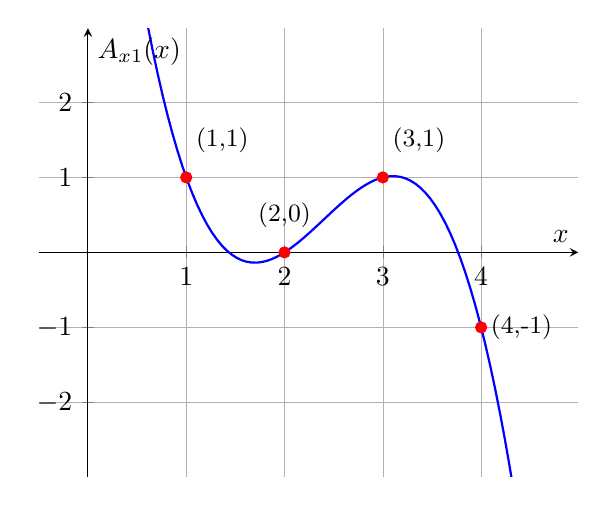
\begin{tikzpicture}
                \begin{axis}[
                    axis lines = middle,
                    xlabel = {$x$},
                    ylabel = {$A_{x1}(x)$},
                    ymin = -2.99, ymax = 2.99,
                    xmin = -0.5, xmax = 4.99,
                    domain = 0:5,
                    samples = 100,
                    ytick = {-3,...,3},
                    xtick = {0,1,...,5},
                    grid = both, 
                    grid style = {line width=.1pt, draw=gray!20},
                    major grid style = {line width=.2pt, draw=gray!60}
                ]
                \addplot[
                    color=blue,
                    thick
                ]
                {-5/6*x^3 + 6*x^2 - 79/6*x + 9};
                \addplot[
                    only marks,
                    mark=*,
                    color=red
                ]
                coordinates {(1,1) (2,0) (3,1) (4,-1)};
        
                \node at (axis cs:1,1.5) [anchor=west] {\small (1,1)};
                \node at (axis cs:2,0.2) [anchor=south] {\small (2,0)};
                \node at (axis cs:3,1.5) [anchor=west] {\small (3,1)};
                \node at (axis cs:4,-1) [anchor=west] {\small (4,-1)};
                
                \end{axis}
            \end{tikzpicture}
    
            \scriptsize\textbf{Illustration:} The Lagrange inteprolation polynomial for points $\{(1,1), (2,0), (3,1), (4,-1)\}$ visualized over $\mathbb{R}$.
        \end{center}
    \end{frame}

    \begin{frame}{Recap. QAP}
        \begin{figure}[H]
            \centering
            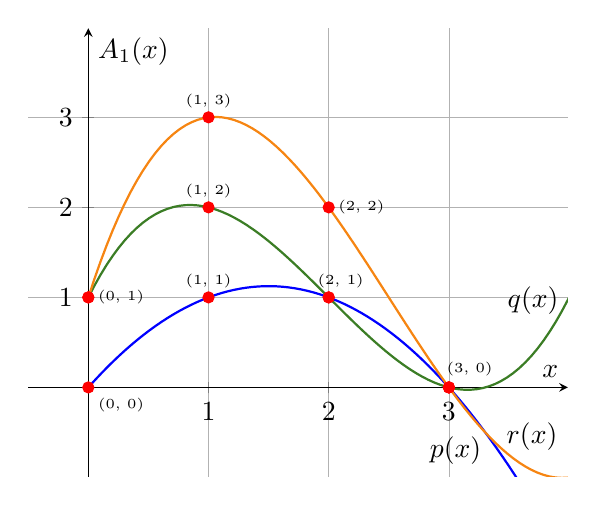
\begin{tikzpicture}
                \begin{axis}[
                    axis lines = middle,
                    xlabel = {$x$},
                    ylabel = {$A_1(x)$},
                    ymin = -0.99, ymax = 3.99,
                    xmin = -0.5, xmax = 3.99,
                    domain = 0:5,
                    samples = 100,
                    ytick = {-1,...,4},
                    xtick = {0,1,...,4},
                    grid = both,
                    grid style = {line width=.1pt, draw=gray!20},
                    major grid style = {line width=.2pt, draw=gray!60}
                ]

                % p(x)
                \addplot[
                    color=blue,
                    thick
                ]
                {3/2*x - 1/2*x^2};
                \addplot[
                    only marks,
                    mark=*,
                    color=red
                ]
                coordinates {(0, 0) (1, 1) (2, 1) (3, 0)};
                \node at (axis cs:3.35,-0.7) [anchor=east] {\text{$p(x)$}};

                \node at (axis cs:0,-0.2) [anchor=west] {\tiny (0, 0)};
                \node at (axis cs:1,1) [anchor=south] {\tiny (1, 1)};
                \node at (axis cs:2.1,1) [anchor=south] {\tiny (2, 1)};
                \node at (axis cs:2.9,0.2) [anchor=west] {\tiny (3, 0)};

                % q(x)
                \addplot[
                    color=OliveGreen,
                    thick
                ]
                {1/3*x^3 - 2*x^2 + 8/3*x + 1};
                \addplot[
                    only marks,
                    mark=*,
                    color=red
                ]
                coordinates {(0,1) (1,2) (2,1) (3, 0)};
                \node at (axis cs:3.7,0.7) [anchor=south] {\text{$q(x)$}};

                \node at (axis cs:0,1) [anchor=west] {\tiny (0, 1)};
                \node at (axis cs:1,2) [anchor=south] {\tiny (1, 2)};

                % r(x)
                \addplot[
                    color=BurntOrange,
                    thick
                ]
                {1/3*x^3 - 5/2*x^2 + 25/6*x + 1};
                \addplot[
                    only marks,
                    mark=*,
                    color=red
                ]
                coordinates {(0,1) (1,3) (2,2) (3, 0)};
                \node at (axis cs:3.4,-0.55) [anchor=west] {\text{$r(x)$}};

                \node at (axis cs:1,3) [anchor=south] {\tiny (1, 3)};
                \node at (axis cs:2,2) [anchor=west] {\tiny (2, 2)};

                \end{axis}
            \end{tikzpicture}
            \caption{Addition of two polynomials}
            \label{fig:example-polynomial-addition}
        \end{figure}
    \end{frame}

    \begin{frame}
        \vspace{-5pt}
        Now, using coefficients encoded with polynomials, we can build a constraint number 
        $x \in \{1, \dots, m\}$ in the next way:
        \vspace{-5pt}
        \begin{align*}
            &(w_1A_1(x) + w_2A_2(x) + \dots + w_nA_n(x)) \times \\
            \times &(w_1B_1(x) + w_2B_2(x) + \dots + w_nB_n(x)) = \\ 
            = &(w_1C_1(x) + w_2C_2(x) + \dots + w_nC_n(x))
            \vspace{-5pt}
        \end{align*}
        
        Or written more concisely:
        \vspace{-5pt}
        \begin{equation*}
            \left( \sum_{i = 1}^{n} w_iA_i(x) \right) \times \left( \sum_{i = 1}^{n} w_iB_i(x) \right) = \left( \sum_{i = 1}^{n} w_iC_i(x) \right)
        \end{equation*}   
        
        \vspace{-5pt}
        \begin{equation*}
            A(x) \times B(x) = C(x)
        \end{equation*}   
    \end{frame}

    \begin{frame}{Recap. QAP}
        Now, we can define a \textbf{master polynomial} $M(x)$, that has zeros at all elements from the set
        $\Omega = \{1,\dots,m\}$
        \vspace{-5pt}
        \begin{equation*}
            M(x) = A(x) \times B(x) - C(x)
            \vspace{-5pt}
        \end{equation*}
        
        It means, that $M(x)$ can be divided by \textbf{vanishing polynomial} $Z_{\Omega}(x)$ without a remainder!
        \vspace{-8pt}
        \begin{equation*}
            Z_{\Omega}(x) = \prod_{i=1}^m (x - i), \qquad \text{$H(x) = \frac{M(x)}{Z_{\Omega}(x)}$ is a polynomial}
            \vspace{-5pt}
        \end{equation*}
    \end{frame}

    \section{Encrypted Verification}

    \begin{frame}{Current Point}
        We've managed to encode into \textbf{a single polynomial} an entire computation (a program),
        of any size, independent of how much data it consumes. \\ 
        \vspace{10pt}
        Now, we need to figure our the protocol, how a prover can succinctly proof the knowledge of
        a correct witness for some circuit to a verifier, additionally, make it zero-knowledge and 
        non-interactive.

        Where the knowledge of the correct witness is a knowledge of the quotient polynomial $H(x)$.
        \begin{equation*}
            M(x) = H(x) \times Z_{\Omega}(x)
        \end{equation*}

        \begin{block}{Remark}
            Further, for brevity, we will denote $Z_{\Omega}(x)$ as $Z(x)$.
        \end{block}
    \end{frame}

    \begin{frame}{Notation Preliminaries: Groups}
        In this section, we will use:
        \begin{itemize}[label=\ding{51}]
            \item Group of points on elliptic curve 
            denoted as $\mathbb{G}$ of prime order $q$ with a generator $g$.
            \item The symmetric pairing function $e: \mathbb{G} \times \mathbb{G} \to \mathbb{G}_T$, where
            $(\mathbb{G}_T, \times)$ is a target group (typically, just a scalar from extension $\mathbb{F}_{p^k}$).
        \end{itemize}
        \begin{alertblock}{Recall}
            The core property of the pairing function $e$ is the \textbf{bilinearity}:
            \begin{equation*}
                e(g^{\alpha}, g^{\beta}) = e(g^{\alpha\beta}, g) = e(g, g^{\alpha\beta}) = e(g,g)^{\alpha\beta}.
            \end{equation*}

            Here, $g^{\alpha}$ is the same as ``scalar multiplication of a generator by a scalar $\alpha \in \mathbb{Z}_q$''.
        \end{alertblock}
    \end{frame}

    \begin{frame}{Notation Preliminaries: QAP}
        Recall that the core equation to be proven:
        \begin{equation*}
            \left( \sum_{i = 1}^{n} w_iA_i(x) \right) \times \left( \sum_{i = 1}^{n} w_iB_i(x) \right) - \left( \sum_{i = 1}^{n} w_iC_i(x) \right) = Z(x)H(x)
        \end{equation*}

        Here, we will change notation a bit: instead of $A$ and $B$, we are going to use $L$ and $R$, while $C$ becomes $O$.

        So equation becomes:
        \begin{equation*}
            \textcolor{oc-indigo-8}{\underbrace{\left( \sum_{i = 1}^{n} w_iL_i(x) \right)}_{\text{left wires encoding}}} \times \textcolor{oc-yellow-8}{\underbrace{\left( \sum_{i = 1}^{n} w_iR_i(x) \right)}_{\text{right wires encoding}}} - \textcolor{oc-green-8}{\underbrace{\left( \sum_{i = 1}^{n} w_iO_i(x) \right)}_{\text{output encodings}}} = Z(x)H(x)
        \end{equation*}
    \end{frame}

    \begin{frame}{Naive Proof}
        Suppose, we are given a circuit $\mathcal{C}$ with a maximum degree $d$ of polynomials
        used underneath.
        
        Thus, all parties additionally know the target polynomial $Z(x)$ and QAP polynomials 
        $\{L_i(x)\}_{i \in [n]}, \{R_i(x)\}_{i \in [n]}, \{O_i(x)\}_{i \in [n]}$, where $n$ is 
        number of witness elements.

        
        \textbf{Prover}
        \vspace{-5pt}
        \begin{itemize}[label=\ding{51}]
            \item \vspace{-3pt} Provides witness $\boldsymbol{w}$ to a Verifier.
        \end{itemize}
        
        \textbf{Verifier}
        \vspace{-5pt}
        \begin{itemize}[label=\ding{51}]
            \item \vspace{-3pt} Checks $\left( \sum_{i = 1}^{n} w_iL_i(x) \right) \times \left( \sum_{i = 1}^{n} w_iR_i(x) \right) = \left( \sum_{i = 1}^{n} w_iO_i(x) \right)$
        \end{itemize}
    \end{frame}

    \begin{frame}{Naive Proof}
        \begin{itemize}
            \item[\ding{55}] Succint
            \item[\ding{51}] Non-Interactive
            \item[\ding{55}] Zero-Knowledge
        \end{itemize}

        
        \vspace{20pt}
        \begin{columns}
            \begin{column}{0.7\textwidth}
                The verifier could actually just run a program that represents a circuit 
                $\mathtt{C}$ on witness data $\boldsymbol{w}$.
            \end{column}

            \begin{column}{0.2\textwidth}
                
\includegraphics[width=\linewidth]{../presentations/images/common/new-moon-with-face.jpg}
            \end{column}
        \end{columns}

        We, definitely, need to encrypt the witness data $\boldsymbol{w}$ somehow...
    \end{frame}

    \begin{frame}
        Let's define the \textit{encryption} operation as follows:
        \vspace{-10pt}
        \begin{equation*}
            \mathsf{Enc}: \mathbb{Z}_q \to \mathbb{G}, \quad \mathsf{Enc}(x) := g^x
            \vspace{-5pt}
        \end{equation*}
        Essentially, $\mathsf{Enc}(p(\tau))$ is the \textbf{KZG Commitment} $\mathsf{com}(p)$. 
        \begin{example}
            Consider the polynomial: $p(x) = x^2 - 5x + 2$, the encryption of $p(\tau)$ can be found as follows:
            {\large
            \begin{equation*}
                \mathsf{Enc}(p(\tau)) = g^{p(\tau)} = g^{\left( \tau^2 - 5\tau + 2 \right)}  = \left( g^{\tau^2} \right)^1 \cdot {\left( g^{\tau^1} \right)}^{-5} \cdot \left(g^{\tau^0}\right)^2
            \end{equation*}}
        \end{example}
        \begin{alertblock}{Question}
            KZG Commitment requires encrypted powers of $\tau$: $\{g^{\tau^i}\}_{i \in [d]}$. But 
            where the prover can take them?
        \end{alertblock}
    \end{frame}

    \begin{frame}{Trusted Setup}
        \textbf{Trusted Party Setup}
        \vspace{-5pt}
        \begin{itemize}[label=\ding{51}]
            \item \vspace{-3pt} Picks a random value $\tau \xleftarrow{R} \mathbb{F}$. 
            \item \vspace{-3pt} Calculates the public parameters $\{g^{\tau^i}\}_{i \in [d]}$.
            \item \vspace{-3pt} \textbf{Deletes} $\tau$ (toxic waste).
            \item \vspace{-3pt} \textbf{Outputs} prover parameters $\mathsf{pp} \gets \{g^{\tau^i}\}_{i \in [d]}$ and verifier parameters $\mathsf{vp} \gets \mathsf{com}(Z)$. 
        \end{itemize} 

        This way, we can find the KZG commitment for each polynomial. For example:
        \begin{equation*}
            \mathsf{com}(L) \triangleq g^{L(\tau)} = g^{\sum_{i=0}^d L_i \tau^i} = \prod_{i=0}^d (g^{\tau^i})^{L_i},
        \end{equation*}
    \end{frame}

    \begin{frame}
        Now, we can calculate the following KZG commitments (or, synonymously, encryptions):
        \begin{equation*}
            g^{L(\tau)}, g^{R(\tau)}, g^{O(\tau)}, g^{H(\tau)}, g^{Z(\tau)}
        \end{equation*}
        But how can we verify $H(x)Z(x) = L(x)R(x) - O(x)$ in the encrypted space? 
        
        Well, first notice that, according to the \textbf{Schwarz-Zippel Lemma}, \textit{with overwhelming probability} the check is equivalent to:
        \begin{equation*}
            L(\tau)R(\tau) = Z(\tau)H(\tau) + O(\tau).
        \end{equation*}
        So, we can check this equality as follows:
        \begin{equation*}
            e(\mathsf{com}(L), \mathsf{com}(R)) = e(\mathsf{com}(Z), \mathsf{com}(H)) \cdot e(\mathsf{com}(O), g),
        \end{equation*}
    \end{frame}

    \begin{frame}
        \scriptsize

        \textbf{Trusted Setup: }
        $\tau \xleftarrow{R} \mathbb{F} \textbf{,} \quad \{g^{\tau^i}\}_{i \in [d]}\textbf{,} \quad g^{Z(\tau)} \textbf{,} \quad \textbf{delete}(\tau)$.
        \vspace{10pt}

        \tikzset{
            arrow/.style={-latex, ultra thick}
        }

        \begin{center}
            \begin{tikzpicture}
                \node[inner sep=0pt, align=center] (prover) at (-3.5, -3) {
                    
\includegraphics[width=2cm]{images/common/prover.png}\\Prover $\mathcal{P}$
                };

                \node[inner sep=0pt, align=center] (verifier) at (4, -3) {
                    
\includegraphics[width=2cm]{images/common/verifier.png}\\Verifier $\mathcal{V}$
                };
                
               
                    \node[inner sep=0pt, align=center] (pdata) at (-3, -0.6) {
                        \begin{minipage}{4cm}
                            \begin{itemize}[label=\ding{51}]
                                \item $H(x) = \frac{L(x) \times R(x) - O(x)}{Z(x)}$.
                                \item {
                                    KZG commitments: 
                                    \vspace{-10pt}
                                    \begin{align*}
                                        \pi_L &\gets \mathsf{com}(L), &\pi_R &\gets \mathsf{com}(R), \\ 
                                        \pi_O &\gets \mathsf{com}(O), &\pi_H &\gets \mathsf{com}(H),
                                    \end{align*}
                                }
                            \end{itemize}
                        \end{minipage}
                    };
                

                
                    \draw[arrow] (prover) -- (verifier) node[midway, above=1mm] {$\boldsymbol{\pi} = (\pi_L,\pi_R,\pi_O,\pi_H)$};
                

                
                    \node[inner sep=0pt, align=center] (vdata) at (5, -1.1) {
                        \begin{minipage}{6cm}
                            \begin{itemize}[label=\ding{51}]
                                \item $e(\pi_L, \pi_R) \xlongequal{?} \\ e(\mathsf{com}(Z), \pi_H) \cdot e(\pi_O, g)$.
                            \end{itemize}
                        \end{minipage}
                    };
                
            \end{tikzpicture}
        \end{center}
    \end{frame}

    \begin{frame}
        \begin{itemize}
            \item[\ding{51}] Succint
            \item[\ding{51}] Non-Interactive
            \item[\ding{51}] Zero-Knowledge 
            \item[\ding{55}] \vspace{7pt} Does it work?
        \end{itemize}
    \end{frame}

    \begin{frame}{Why it doesn't work??}\begin{adjustwidth}{-5mm}{0mm}
        \scriptsize

        \textbf{Trusted Setup: }
        $\tau \xleftarrow{R} \mathbb{F} \textbf{,} \quad \{g^{\tau^i}\}_{i \in [d]}\textbf{,} \quad g^{Z(\tau)}\textbf{,}$ \textbf{delete}($\tau$).
        \vspace{10pt}

        \tikzset{
            arrow/.style={-latex, ultra thick}
        }

        \begin{center}
            \begin{tikzpicture}
                \node[inner sep=0pt, align=center] (prover) at (-3.5, -2.4) {
                    
\includegraphics[width=2cm]{images/common/prover.png}\\Prover $\mathcal{P}$
                };

                \node[inner sep=0pt, align=center] (verifier) at (4, -2.4) {
                    
\includegraphics[width=2cm]{images/common/verifier.png}\\Verifier $\mathcal{V}$
                };
                
                \node[inner sep=0pt, align=center] (pdata) at (-2.3, 0) {
                    \begin{minipage}{6cm}
                        \begin{itemize}[label=\ding{51}]
                            \item $H^{\prime}(x) \xleftarrow{R} \mathbb{F}[x], \quad M^{\prime}(x) = Z(x) \times H^{\prime}(x)$.
                            \item Finds $L^{\prime}(x), R^{\prime}(x), O^{\prime}(x)$ such that: \\ $L^{\prime}(x) \times R^{\prime}(x) - O^{\prime}(x) = M^{\prime}(x)$
                            \item {
                                KZG commitments: 
                                \vspace{-10pt}
                                \begin{align*}
                                    \pi_{L^{\prime}(x)} &\gets \mathsf{com}(L^{\prime}(x)), &\pi_{R^{\prime}(x)} &\gets \mathsf{com}(R^{\prime}(x)), \\ 
                                    \pi_{O^{\prime}(x)} &\gets \mathsf{com}(O^{\prime}(x)), &\pi_{H^{\prime}(x)} &\gets \mathsf{com}(H^{\prime}(x)),
                                \end{align*}
                            }
                        \end{itemize}
                    \end{minipage}
                };

                \draw[arrow] (prover) -- (verifier) node[midway, above=1mm] {$\boldsymbol{\pi} = (\pi_{L^{\prime}(x)},\pi_{R^{\prime}(x)},\pi_{O^{\prime}(x)},\pi_{H^{\prime}(x)})$};

                \node[inner sep=0pt, align=center] (vdata) at (5.1, -0.6) {
                    \begin{minipage}{6cm}
                        \begin{itemize}[label=\ding{51}]
                            \item $e(\pi_{L^{\prime}(x)}, \pi_{R^{\prime}(x)}) \xlongequal{?} \\ e(\mathsf{com}(Z), \pi_H) \cdot e(\pi_{O^{\prime}(x)}, g)$.
                        \end{itemize}
                    \end{minipage}
                };
            \end{tikzpicture}
        \end{center}

        
        \begin{block}{Problem}
            Prover isn't forced to use the values from the trusted setup.
        \end{block}
    \end{adjustwidth}\end{frame}

    \begin{frame}{Proof Of Exponent}
        \scriptsize

        \textbf{Trusted Setup: }
        $\tau, \textcolor{green!50!black}{\alpha} \xleftarrow{R} \mathbb{F} \textbf{,} \quad \{ \{g^{\tau^i}, \textcolor{green!50!black}{g^{\alpha \tau^i}}\}_{i \in [d]} \} \textbf{,} \quad \{g^{Z(\tau)}, \textcolor{green!50!black}{g^{\alpha}}\}\textbf{,} \quad \textbf{delete}(\tau, \textcolor{green!50!black}{\alpha})$.
        \vspace{10pt}

        \tikzset{
            arrow/.style={-latex, ultra thick}
        }

        \begin{center}
            \begin{tikzpicture}
                \node[inner sep=0pt, align=center] (prover) at (-3.5, -3) {
                    
\includegraphics[width=2cm]{images/common/prover.png}\\Prover $\mathcal{P}$
                };

                \node[inner sep=0pt, align=center] (verifier) at (4, -3) {
                    
\includegraphics[width=2cm]{images/common/verifier.png}\\Verifier $\mathcal{V}$
                };
                
                \node[inner sep=0pt, align=center] (pdata) at (-3, -0.6) {
                    \begin{minipage}{4cm}
                        {\tiny\begin{itemize}[label=\ding{51}]
                            \item $H(x) = \frac{L(x) \times R(x) - O(x)}{Z(x)}$.
                            \item {
                                KZG commitments: 
                                \vspace{-8pt}
                                \begin{align*}
                                    \pi_L &\gets g^{L(\tau)}, \quad & \textcolor{green!50!black}{\pi_L'} &\gets \textcolor{green!50!black}{g^{\alpha L(\tau)}},\\[-2pt]
                                    \pi_R &\gets g^{R(\tau)}, \quad & \textcolor{green!50!black}{\pi_R'} &\gets g^{\alpha R(\tau)},\\[-2pt]
                                    \pi_O &\gets g^{O(\tau)}, \quad & \textcolor{green!50!black}{\pi_O'} &\gets g^{\alpha O(\tau)},\\[-2pt]
                                    \pi_H &\gets g^{H(\tau)}, \quad & \textcolor{green!50!black}{\pi_H'} &\gets g^{\alpha H(\tau)}.
                                \end{align*}
                            }
                        \end{itemize}}
                    \end{minipage}
                };
            
                \draw[arrow] (prover) -- (verifier) node[midway, above=1mm] {$\boldsymbol{\pi} = (\pi_L,\pi_R,\pi_O,\pi_H,\textcolor{green!50!black}{\pi_L',\pi_R',\pi_O',\pi_H'})$};

                \node[inner sep=0pt, align=center] (vdata) at (5, -0.6) {
                    \begin{minipage}{4cm}
                        {\tiny\begin{itemize}[label=\ding{51}]
                            \item $e(\pi_L, \pi_R) \xlongequal{?}\\ e(\mathsf{com}(Z), \pi_H) \cdot e(\pi_O, g)$.
                            \item \textcolor{green!50!black}{
                                Proof of Exponent:
                                \vspace{-8pt}
                                \begin{align*}
                                    e(\pi_L, g^{\alpha}) &= e(\pi_L', g), \qquad\qquad\qquad\\[-2pt] %quads are to adjust spacing on the slide
                                    e(\pi_R, g^{\alpha}) &= e(\pi_R', g), \\[-2pt]
                                    e(\pi_O, g^{\alpha}) &= e(\pi_O', g), \\[-2pt]
                                    e(\pi_H, g^{\alpha}) &= e(\pi_H', g).
                                \end{align*}
                            }
                        \end{itemize}}
                    \end{minipage}
                };
            \end{tikzpicture}
        \end{center}
    \end{frame}

    \begin{frame}{Including PoE}
        \begin{itemize}
            \item[\ding{51}] Succint
            \item[\ding{51}] Non-Interactive
            \item[\ding{51}] Zero-Knowledge 
            \item[\ding{55}] Sound
        \end{itemize}

        
        \vspace{15pt}
        \begin{block}{Problem}
            There is no guarantee that the same witness $\mathbf{w}$ was used to calculate all the commitments $\pi_L, \pi_R, \pi_O, \pi_H$.
        \end{block}
    \end{frame}

    \section{Make It Sound}

    \begin{frame}{Additional Optimization}
        Recal that:
        \begin{equation*}
            L(x) = \sum_{i=0}^n w_iL_i(x), \quad R(x) = \sum_{i=0}^n w_i R_i(x), \quad O(x) = \sum_{i=0}^n w_iO_i(x).
        \end{equation*}

        

        Here public data is:
        \begin{equation*}
            \{L_i(x)\}_{i \in [n]}, \{R_i(x)\}_{i \in [n]}, \{O_i(x)\}_{i \in [n]}
        \end{equation*}

        
        
        Moreover, it's defined only by the circuit and trusted setup, thus, it can calculated before proof generation as a part of the trusted setup.
    \end{frame}

    \begin{frame}{Additional Optimization}
        Updated Trusted Setup:
        \vspace{-10pt}
        {\scriptsize \begin{align*}
            \{g^{\tau^i}\}_{i \in [d]}&, \quad \{g^{\alpha \tau^i}\}_{i \in [d]}, \\
            \textcolor{green!50!black}{\{g^{L_i(\tau)}\}_{i \in [n]}}&, \quad \textcolor{green!50!black}{\{g^{\alpha L_i(\tau)}\}_{i \in [n]}},\\ 
            \textcolor{green!50!black}{\{g^{R_i(\tau)}\}_{i \in [n]}}&, \quad \textcolor{green!50!black}{\{g^{\alpha R_i(\tau)}\}_{i \in [n]}},\\
            \textcolor{green!50!black}{\{g^{O_i(\tau)}\}_{i \in [n]}}&, \quad \textcolor{green!50!black}{\{g^{\alpha O_i(\tau)}\}_{i \in [n]}}  
        \end{align*}}
       
        
        
        Consider the polynomial $L(x) = \sum_{i=0}^n w_iL_i(x)$. 
        
        
        
        $\mathcal{P}$ can compute the KZG commitment $\pi_L$ and its PoE $\pi_L'$ as follows:
        \begin{align*}
            \pi_L &\triangleq g^{L(\tau)} = g^{\sum_{i=0}^n w_i L_i(\tau)} = \prod_{i=0}^n (g^{L_i(\tau)})^{w_i}, \\
            \pi_L' &\triangleq g^{\alpha L(\tau)} = g^{\alpha \sum_{i=0}^n w_i L_i(\tau)} = \prod_{i=0}^n (g^{\alpha L_i(\tau)})^{w_i}.
        \end{align*}
    \end{frame}

    \begin{frame}{Witness Consistency Check}
        
        To prove that the same $\mathbf{w}$ is used in all commitments, we need some ``checksum''
        term that will somehow combine all polynomials $L(x)$, $R(x)$, and $O(x)$ with the witness
        $\mathbf{w}$.

        
        We can do so by proving the next simple statement:
        \vspace{-5pt}
        \begin{equation*}
            g^{L(\tau) + R(\tau) + O(\tau)} =  \prod_{i=1}^n {\left(g^{L_i(\tau) + R_i(\tau) + O_i(\tau)}\right)}^{w_i}
            \vspace{-5pt}
        \end{equation*}
        
        And we already know how to do that --- POE!
    \end{frame}

    \begin{frame}{Witness Consistency Check}
        Let's introduce one more coefficient...
        \vspace{-5pt}
        \begin{equation*}
            \beta \xleftarrow{R} \mathbb{F}
            \vspace{-5pt}
        \end{equation*}
        
        Extended trusted setup contains additional values:
        \vspace{-5pt}
        \begin{equation*}
            g^{\beta}, \quad \{g^{\beta(L_i(\tau) + R_i(\tau) + O_i(\tau))}\}_{i \in \left[ n \right]}
            \vspace{-5pt}
        \end{equation*}
        
        Prover needs to calculate $\pi_{\beta}$:
        \vspace{-5pt}
        \begin{equation*}
            \pi_{\beta} \gets g^{\beta(L(\tau) + R(\tau) + O(\tau))} =  \prod_{i=1}^{n} g^{\beta(L_i(\tau) + R_i(\tau) + O_i(\tau))}g^{w_i}\
        \end{equation*}
        
        And easy check for verifier:
        \vspace{-5pt}
        \begin{equation*}
            e(\pi_L\pi_R\pi_O, g^{\beta}) = e(\pi_{\beta}, g).
        \end{equation*}
    \end{frame}

    \begin{frame}{One more time... that doesn't work}
        If the witness is consistent, the following condition must hold:
        \vspace{-3pt}
        {\small \begin{equation*}
            (w_{L,i}L_i(\tau) + w_{R,i}R_i(\tau) + w_{O,i}O_i(\tau))\beta = w_i\beta(L_i(\tau) + R_i(\tau) + O_i(\tau)) \quad \forall i \in [n]
            \vspace{-10pt}
        \end{equation*}}
        
        
        But, what if $L_i \equiv R_i$. Let's call them $q$, thus:
        \vspace{-3pt}
        \begin{equation*}
            (w_{L,i} + w_{R,i})q + w_{O,i}O_i(\tau)= w_{\beta,i}(2q + O_i(\tau)) \quad \forall i \in [n]
            \vspace{-10pt}
        \end{equation*}

        
        The adversary can choose $w_{L,i}$, $w_{R,i}$ and $w_{O,i}$ such that:
        \vspace{-5pt}
        \begin{equation*}
            w_i := w_{O,i} \quad \text{and} \quad w_{L,i}=2w_{O,i} - w_{R,i}
            \vspace{-5pt}
        \end{equation*} 

        
        \begin{example}
            \begin{equation*}
                w = w_O = 5, \quad w_L = 7, \quad w_R = 3
                \vspace{-25pt}
            \end{equation*}

            \begin{align*}
                (7 + 3)q + 5O(\tau) = 5(2q + O(\tau)) \\
                10q + 5O(\tau) = 10q + 5O(\tau)
            \end{align*}
        \end{example}
    \end{frame}

    \begin{frame}{More coefficients!}
        The main problem is that if $R_i \equiv L_i$ then $\beta R_i \equiv \beta L_i$.

        Let's fix that by introducing a separate $\beta$ coefficients for $L$, $R$ and $O$.
        \begin{equation*}
            \left( \beta_L, \beta_R, \beta_O \right) \xleftarrow{R} \mathbb{F}^3
            \vspace{-5pt}
        \end{equation*}
        
        
        Therefore, $\beta_R R_i \neq \beta_L L_i$ even if $R_i \equiv L_i$, so the previous hack doesn't work.

        So, finally, the trusted setup is updated with:
        \vspace{-5pt}
        \begin{equation*}
            g^{\beta_L}, g^{\beta_R}, g^{\beta_O}, \{g^{\left( \beta_LL_i(\tau) + \beta_RR_i(\tau) + \beta_OO_i(\tau) \right)}\}_{i \in \left[ n \right]}
            \vspace{-5pt}
        \end{equation*}

        
        Verification:
        \vspace{-5pt}
        \begin{equation*}
            e(\pi_L, g^{\beta_L}) \cdot e(\pi_R, g^{\beta_R}) \cdot e(\pi_O, g^{\beta_O}) = e(\pi_{\beta}, g)
        \end{equation*}
    \end{frame}

    \begin{frame}{Even more coefficients!}
        As the adversary has an access to the public $g^{\beta_L}$, $g^{\beta_R}$, $g^{\beta_O}$ he still can cheat verifier by calculating modified $\pi_{\beta}$.

        \begin{example}
            \small
            Consider a constraint $w_1 \times w_1 = w_2$. Let's try to assign $2$ and $5$ for $w_1$ in a single constraint. As $2 \times 5 = 10$, the $w_2$ should contains value $10$.
            \vspace{-5pt}
            \begin{equation*}
                \mathbf{w} = (w_1, w_2) = (2, 10)
                \vspace{-5pt}
            \end{equation*}
            
            The next QAP can be built:
            \vspace{-5pt}
            \begin{align*}
                L(x) &= 2L_1(x) + 10L_2(x) \\
                R(x) &= 2R_1(x) + 3 + 10R_2(x) \\
                O(x) &= 2O_1(x) + 10O_2(x)
            \end{align*}
            
            Compute $\pi_{\beta}$ as:
            \vspace{-5pt}
            \begin{equation*}
                (g^{\left( \beta_LL_1(\tau) + \beta_RR_1(\tau) + \beta_OO_1(\tau) \right)})^2 \cdot (g^{\beta_R})^3 \cdot (g^{\left( \beta_LL_2(\tau) + \beta_RR_2(\tau) + \beta_OO_2(\tau) \right)})^{10} 
            \end{equation*}
        \end{example}
    \end{frame}

    \begin{frame}{Even more coefficients!}
        To prevent this, let's introduce... one more coefficient!
        \vspace{-5pt}

        \begin{equation*}
            \gamma \xleftarrow{R} \mathbb{F}
            \vspace{-5pt}
        \end{equation*}

        
        So, finally... the trusted setup is updated with:
        \vspace{-5pt}
        \begin{equation*}
            g^{\gamma}, g^{\beta_L}, g^{\beta_R}, g^{\beta_O}, \{g^{\left( \beta_LL_i(\tau) + \beta_RR_i(\tau) + \beta_OO_i(\tau) \right)}\}_{i \in \left[ n \right]}
            \vspace{-5pt}
        \end{equation*}

        
        Proving process isn't changed, unlike verification:
        \begin{equation*}
            e(\pi_L, g^{\beta_L\gamma}) \cdot e(\pi_R, g^{\beta_R\gamma}) \cdot e(\pi_O, g^{\beta_O\gamma}) = e(\pi_{\beta}, g^{\gamma})
        \end{equation*}

        That makes it unfeasible to cheat.
    \end{frame}

    \begin{frame}{Sound SNARK Protocol}
        \scriptsize

        \textbf{Trusted Setup: }
        $\tau, \alpha, \textcolor{green!50!black}{\beta_L, \beta_R, \beta_O, \gamma} \xleftarrow{R} \mathbb{F} \textbf{,} \quad \{ \{g^{\tau^i}, g^{\alpha \tau^i} \}_{i \in [d]}\textbf{,} \quad \textcolor{green!50!black}{\{g^{\left( \beta_LL_i(\tau) + \beta_RR_i(\tau) + \beta_OO_i(\tau) \right)}\}_{i \in \left[ n \right]}} \} \textbf{,}$
        $\{ g^{Z(\tau)}, g^{\alpha}, \textcolor{green!50!black}{g^{\beta_L}, g^{\beta_R}, g^{\beta_O}, g^{\beta_L\gamma}, g^{\beta_R\gamma}, g^{\beta_O\gamma}, g^{\gamma}}\}\textbf{,} \quad \textbf{delete}(\tau, \alpha, \textcolor{green!50!black}{\beta_L, \beta_R, \beta_O, \gamma})$.
        \vspace{10pt}

        \tikzset{
            arrow/.style={-latex, ultra thick}
        }

        \begin{center}
            \begin{tikzpicture}
                \node[inner sep=0pt, align=center] (prover) at (-3.5, -3) {
                    
\includegraphics[width=2cm]{images/common/prover.png}\\Prover $\mathcal{P}$
                };

                \node[inner sep=0pt, align=center] (verifier) at (4, -3) {
                    
\includegraphics[width=2cm]{images/common/verifier.png}\\Verifier $\mathcal{V}$
                };
                
                \node[inner sep=0pt, align=center] (pdata) at (-3, 0) {
                    \begin{minipage}{4cm}
                        {\tiny\begin{itemize}[label=\ding{51}]
                            \item $H(x) = \frac{L(x) \times R(x) - O(x)}{Z(x)}$.
                            \item {
                                KZG commitments: 
                                \vspace{-8pt}
                                \begin{align*}
                                    \pi_L &\gets g^{L(\tau)}, \quad &\pi_L' &\gets g^{\alpha L(\tau)},\\[-2pt]
                                    \pi_R &\gets g^{R(\tau)}, \quad &\pi_R' &\gets g^{\alpha R(\tau)},\\[-2pt]
                                    \pi_O &\gets g^{O(\tau)}, \quad &\pi_O' &\gets g^{\alpha O(\tau)},\\[-2pt]
                                    \pi_H &\gets g^{H(\tau)}, \quad &\pi_H' &\gets g^{\alpha H(\tau)}.
                                \end{align*}
                                \vspace{-16pt}
                            }
                            \item \textcolor{green!50!black}{
                                \vspace{-18pt}
                                $\textcolor{green!50!black}{\pi_{\beta} \gets g^{\beta_LL(\tau) + \beta_RR(\tau) + \beta_OO(\tau)}}$
                            }
                        \end{itemize}}
                    \end{minipage}
                };
            
                \draw[arrow] (prover) -- (verifier) node[midway, above=1mm] {$\boldsymbol{\pi} = (\pi_L,\pi_R,\pi_O,\pi_H,\pi_L',\pi_R',\pi_O',\pi_H',\textcolor{green!50!black}{\pi_{\beta}})$};

                \node[inner sep=0pt, align=center] (vdata) at (5, -0.2) {
                    \begin{minipage}{5cm}
                        {\tiny\begin{itemize}[label=\ding{51}]
                            \item $e(\pi_L, \pi_R) \xlongequal{?}\\ e(\mathsf{com}(Z), \pi_H) \cdot e(\pi_O, g)$.
                            \item {
                                Proof of Exponent:
                                \vspace{-8pt}
                                \begin{align*}
                                    e(\pi_L, g^{\alpha}) &= e(\pi_L', g), \qquad\qquad\qquad\\[-2pt] %quads are to adjust spacing on the slide
                                    e(\pi_R, g^{\alpha}) &= e(\pi_R', g), \\[-2pt]
                                    e(\pi_O, g^{\alpha}) &= e(\pi_O', g), \\[-2pt]
                                    e(\pi_H, g^{\alpha}) &= e(\pi_H', g).
                                \end{align*}
                                \vspace{-16pt}
                            }
                            \item \textcolor{green!50!black}{
                                $e(\pi_L, g^{\gamma\beta_L}) \cdot e(\pi_R, g^{\gamma\beta_R}) \cdot \\ \cdot e(\pi_O, g^{\gamma\beta_O}) = e(\pi_{\beta}, g^{\gamma})$
                            }
                        \end{itemize}}
                    \end{minipage}
                };
            \end{tikzpicture}
        \end{center}
    \end{frame}

    \section{Make it Zero-Knowledge}

    \begin{frame}{Why we need modifications?}
        \begin{alertblock}{Question}
            \begin{itemize}[label=\ding{228}]
                \item According to the security assumptions, given any element of our proof $\boldsymbol{\pi}$, it is impossible to restore the witness $\boldsymbol{w}$.
                \item Well, that is true, but does it guarantee that no other information about $\boldsymbol{w}$ is \textbf{not leaked}?
            \end{itemize}

            It does not! For example, given $\boldsymbol{\pi}$, I can check if $L(x) = 10R(x)$. 
            
            How? Simply check
            \begin{equation*}
                \pi_L \xlongequal{?} \pi_R^{10}.
            \end{equation*}

             This works since $\pi_L = g^{L(\tau)}$ and $\pi_R = g^{R(\tau)}$, so
            \begin{equation*}
                \pi_L = \pi_R^{10} \Leftrightarrow g^{L(\tau)} = g^{10R(\tau)} \Leftrightarrow L(\tau) = 10R(\tau) \Leftrightarrow L(x) = 10R(x)
            \end{equation*}
        \end{alertblock}
    \end{frame}

    \begin{frame}{How do we fix that? Analysis}
        \begin{block}{Analysis}
            \begin{itemize}[label=\ding{228}]
                \item Currently, proof consists of four ingredients: $\pi_L, \pi_R, \pi_O, \pi_H$, and their corresponding PoEs. 
                \item But, current construction creates some ``connection'' between these ingredients. For example, $\pi_L^{101} = \pi_R$ reveals whether $101L(x)=R(x)$ or $\pi_L\pi_O=\pi_R$ whether $L(x) + O(x) = R(x)$. 
                \item Therefore, the prover must add some ``noise'' to the proof, so that the verifier can't use the proof to extract any information about the witness. The randomness of prover is kept secret. 
                \item Simultaneously, this noise would still make the same proof checkable by already defined verification equations.
            \end{itemize}
        \end{block}

        \begin{alertblock}{Question}
            So how to we represent such ``noise'' with preserving ``homomorphic'' properties of the proof?
        \end{alertblock}
    \end{frame}

    \begin{frame}{How do we fix that? Doing stuff}
        \begin{block}{Idea \#1}
            Let prover pick random values $\delta_R, \delta_O, \delta_L, \delta_H \xleftarrow{R} \mathbb{F}$ and calculate the ``distorted'' values:
            \begin{equation*}
                \pi_L \gets g^{L(\tau) + \delta_L}, \quad \pi_R \gets g^{R(\tau) + \delta_R}, \quad \text{same for $\pi_O, \pi_H$}
            \end{equation*}
            \textbf{Problem (informally):} To make previous verification mechanism work, $\delta_H$ must be picked ``carefully''. However, it's impossible to do so with this construction.
        \end{block}

        \begin{block}{Idea \#2}
            Let prover pick random values $\delta_R, \delta_O, \delta_L \xleftarrow{R} \mathbb{F}$ and calculate:
            \begin{equation*}
                \pi_L \gets g^{L(\tau) + \delta_L Z(\tau)}, \quad \pi_R \gets g^{R(\tau) + \delta_R Z(\tau)}, \quad \pi_O \gets g^{O(\tau) + \delta_O Z(\tau)}
            \end{equation*}
        \end{block}
    \end{frame}

    \begin{frame}{Making Idea Practical}
        This expression can be easily evaluated. For example,
        \begin{equation*}
            \pi_L = g^{L(\tau)} \cdot \left(g^{Z(\tau)}\right)^{\delta_L} = \mathsf{com}(L) \cdot \mathsf{com}(Z)^{\delta_L}
        \end{equation*}

        \begin{alertblock}{Problem}
            However, the verifier can't check the equation $e(\pi_L, \pi_R) = e(\mathsf{com}(Z), \pi_H) \cdot e(\pi_O, g)$ anymore. 
        \end{alertblock}

        \begin{block}{Idea \#3}
            Our ``noise'' must be controlled! This can be achieved by calculating $\pi_H$ as $g^{H(\tau) + \Delta_H}$ where $\Delta_H$ depends on $\delta_L, \delta_R, \delta_O$ (and possibly other public parameters).    
        \end{block}
    \end{frame}

    \begin{frame}{Making Idea Practical}
        Check $e(\pi_L, \pi_R) = e(\mathsf{com}(Z), \pi_H) \cdot e(\pi_O, g)$ is now equivalent to:
        \begin{equation*}
            (L(x) + \delta_L Z(x))(R(x) + \delta_R Z(x)) = (H(x) + \Delta_H)Z(x) + (O(x) + \delta_O Z(x)),
        \end{equation*}
        
         which, by expanding, gives us the following equation:
        \begin{align*}
            \cancel{L(x)R(x)} + \delta_R L(x)Z(x) + \delta_L Z(x)R(x) + \delta_L \delta_R Z(x)^2 \\= \cancel{H(x)Z(x) + O(x)} + \Delta_HZ(x) + \delta_O Z(x)
        \end{align*}
        
         where we can cancel out $L(x)R(x)$ and $H(x)Z(x) + O(x)$ terms since they are equal based on initial construction. This way, we get the following expression for $\Delta_H$:
        \begin{equation*}
            \boxed{\Delta_H = \delta_O + \delta_R L(x) + \delta_L R(x) + \delta_L \delta_R Z(x)}
        \end{equation*}
    \end{frame}

    \begin{frame}{Witness consistency proof}
        Finally, let us not forget about $\pi_{\beta}$! Previously, we had:
        \begin{equation*}
            \pi_{\beta} = g^{\beta_LL(\tau) + \beta_RR(\tau) + \beta_OO(\tau)}
        \end{equation*}
         Now, we change: 
        \begin{itemize}[label=\ding{228}]
            \item $L(\tau) \mapsto L(\tau) + \delta_L Z(\tau)$
            \item $R(\tau) \mapsto R(\tau) + \delta_R Z(\tau)$
            \item $O(\tau) \mapsto O(\tau) + \delta_O Z(\tau)$
        \end{itemize}
        
         Therefore, our new $\pi_{\beta}$ becomes:
        \begin{equation*}
            \pi_{\beta} = \textcolor{green!50!black}{\left(g^{\beta_LZ(\tau)}\right)^{\delta_L}\left(g^{\beta_R Z(\tau)}\right)^{\delta_R}\left(g^{\beta_O Z(\tau)}\right)^{\delta_O}}g^{\beta_L L(\tau) + \beta_R R(\tau) + \beta_O O(\tau)}
        \end{equation*}
    \end{frame}

    \begin{frame}{Overall protocol}
        \scriptsize

        \textbf{Trusted Setup: }
        $\tau, \alpha, \beta_L, \beta_R, \beta_O, \gamma \xleftarrow{R} \mathbb{F} \textbf{,} \quad \{ \{g^{\tau^i}, g^{\alpha \tau^i} \}_{i \in [d]}\textbf{,} \quad \{\textcolor{green!50!black}{g^{\beta_LL_i(\tau)}, g^{\beta_RR_i(\tau)}, g^{\beta_OO_i(\tau)}}\}_{i \in \left[ n \right]} \} \textbf{,}$
        $\{ g^{Z(\tau)}, g^{\alpha}, g^{\beta_L}, g^{\beta_R}, g^{\beta_O}, g^{\beta_L\gamma}, g^{\beta_R\gamma}, g^{\beta_O\gamma}, g^{\gamma}\}\textbf{,} \quad \textbf{delete}(\tau, \alpha, \beta_L, \beta_R, \beta_O, \gamma)$.
        \vspace{10pt}

        \tikzset{
            arrow/.style={-latex, ultra thick}
        }

        \begin{center}
            \begin{tikzpicture}
                \node[inner sep=0pt, align=center] (prover) at (-3.5, -3) {
                    
\includegraphics[width=2cm]{images/common/prover.png}\\Prover $\mathcal{P}$
                };

                \node[inner sep=0pt, align=center] (verifier) at (4, -3) {
                    
\includegraphics[width=2cm]{images/common/verifier.png}\\Verifier $\mathcal{V}$
                };
                
                \node[inner sep=0pt, align=center] (pdata) at (-3, 0) {
                    \begin{minipage}{4cm}
                        {\tiny\begin{itemize}[label=\ding{51}]
                            \item $H(x) = \frac{L(x) \times R(x) - O(x)}{Z(x)}$.
                            \item {
                                Sample $\delta_L,\delta_R,\delta_O \xleftarrow{R} \mathbb{F}$, compute: 
                                \vspace{-8pt}
                                \begin{align*}
                                    \pi_L \gets g^{L(\tau)}\textcolor{green!50!black}{(g^{Z(\tau)})^{\delta_L}}, \pi_L' \gets g^{\alpha L(\tau)}\textcolor{green!50!black}{(g^{\alpha Z(\tau)})^{\delta_L}},\\[-2pt]
                                    \pi_R \gets g^{R(\tau)}\textcolor{green!50!black}{(g^{Z(\tau)})^{\delta_R}}, \pi_R' \gets g^{\alpha R(\tau)}\textcolor{green!50!black}{(g^{\alpha Z(\tau)})^{\delta_R}},\\[-2pt]
                                    \pi_O \gets g^{O(\tau)}\textcolor{green!50!black}{(g^{Z(\tau)})^{\delta_O}}, \pi_O' \gets g^{\alpha O(\tau)}\textcolor{green!50!black}{(g^{\alpha Z(\tau)})^{\delta_O}},\\[-2pt]
                                    \pi_H \gets g^{H(\tau)}\textcolor{green!50!black}{(g^{\delta_O})(g^{R(\tau)})^{\delta_L}(g^{L(\tau)})^{\delta_R}(g^{Z(\tau)})^{\delta_L\delta_R}}
                                \end{align*}
                                \vspace{-16pt}
                            }
                            
                                \vspace{-5pt}
                                $\pi_{\beta} = \dots$
                            
                        \end{itemize}}
                    \end{minipage}
                };
            
                \draw[arrow] (prover) -- (verifier) node[midway, above=1mm] {$\boldsymbol{\pi} = (\pi_L,\pi_R,\pi_O,\pi_H,\pi_L',\pi_R',\pi_O',\pi_H',\pi_{\beta})$};

                \node[inner sep=0pt, align=center] (vdata) at (5, -0.2) {
                    \begin{minipage}{5cm}
                        {\tiny\begin{itemize}[label=\ding{51}]
                            \item $e(\pi_L, \pi_R) \xlongequal{?}\\ e(\mathsf{com}(Z), \pi_H) \cdot e(\pi_O, g)$.
                            \item {
                                Proof of Exponent:
                                \vspace{-8pt}
                                \begin{align*}
                                    e(\pi_L, g^{\alpha}) &= e(\pi_L', g), \qquad\qquad\qquad\\[-2pt] %quads are to adjust spacing on the slide
                                    e(\pi_R, g^{\alpha}) &= e(\pi_R', g), \\[-2pt]
                                    e(\pi_O, g^{\alpha}) &= e(\pi_O', g), \\[-2pt]
                                    e(\pi_H, g^{\alpha}) &= e(\pi_H', g).
                                \end{align*}
                                \vspace{-16pt}
                            }
                            \item $e(\pi_L, g^{\gamma\beta_L}) \cdot e(\pi_R, g^{\gamma\beta_R}) \cdot \\ \cdot e(\pi_O, g^{\gamma\beta_O}) = e(\pi_{\beta}, g^{\gamma})$
                        \end{itemize}}
                    \end{minipage}
                };
            \end{tikzpicture}
        \end{center}
    \end{frame}

    \section{Real Protocols}
    \begin{frame}{Complexity of the Basic Protocol}
        \begin{block}{Overall Complexity}
            Suppose circuit consists of $n$ gates. Then, the complexity of the basic protocol is as follows:
            \begin{itemize}
                \item \textbf{Proof Size:} $O(1)$ --- constant number of group elements.
                \item \textbf{Setup Time:} $O(n)$ --- calculating powers of $\tau$, evaluations at $\tau$.
                \item \textbf{Prover Time:} $O(n \log n)$ --- using FFT and wise choice of $\Omega$.
                \item \textbf{Verifier Time:} $O(1)$ --- constant number of pairings.
            \end{itemize}
        
            However, $O(1)$ is not very descriptive for proof and verifier complexities, so let us provide a more detailed analysis. 
            \begin{itemize}
                \item \textbf{Proof Size:} 9 $\mathbb{G}$ group elements.
                \item \textbf{Verifier Time:} 15 pairings.
            \end{itemize}
        \end{block}

        We can do better!
    \end{frame}

    \begin{frame}{Pinocchio Protocol}
        \begin{block}{Idea}
            In toxic waste, include $\rho_L,\rho_R \xleftarrow{R} \mathbb{F}$, set $\rho_O \gets \rho_L\rho_R$, and define the following generators:
            \begin{equation*}
                g_L \gets g^{\rho_L}, \quad g_R \gets g^{\rho_R}, \quad g_O \gets g^{\rho_O}
            \end{equation*}
        \end{block}
        
        \begin{alertblock}{Reason}
            Such choice of generators reduce 15 pairings to \textbf{11 pairings}. Additionally, we have only \textbf{8 group elements} in the proof.
        \end{alertblock}
    \end{frame}

    \begin{frame}{Groth16 Protocol}
        \begin{block}{Idea: Generic Group Model}
            Use \textbf{Generic Group Model} (GGM) technique. Simply put, GGM allows the adversary to only make \textbf{oracle requests} to compute the group operations. For example, having a set $\{g^{\alpha R_i(\tau)}\}_{i \in [d]}$, adversary can compute only linear combinations of these values. In the particular case of Groth16, instead of considering $L_i(x)$, $R_i(x)$, and $O_i(x)$ separately, we construct their linear combinations as $Q_i(x) := \beta L_i(x) + \alpha R_i(x) + O_i(x)$, where $\alpha$ and $\beta$ are toxic parameters.
        \end{block}
    \end{frame}

    \begin{frame}{Groth16 Protocol: Setup Procedure}
        The proving key is formed as follows:
        \begin{align*}
            \mathsf{pp} &\gets \Big(g_1^{\alpha},g_1^{\beta},g_1^{\delta},\left\{g_1^{\tau^i},\frac{\beta L_i(\tau) + \alpha R_i(\tau) + O_i(\tau)}{\gamma}, \frac{\tau^i Z(\tau)}{\delta}\right\}_{i \in [n]}, \\
            &g_2^{\beta}, g_2^{\delta}, g_2^{\gamma}, \{g_2^{\tau^i}\}_{i \in [d]}\Big)
        \end{align*}
    \end{frame}

    \begin{frame}{Groth16 Protocol: Proving Procedure}
        Sample random $\delta_L,\delta_R \xleftarrow{R} \mathbb{F}$ and compute the following values:
        \begin{gather*}
            \pi_L \gets g_1^{\alpha + \sum_{i=1}^n w_iL_i(\tau) + \delta_L\delta}, \quad \pi_R \gets g_2^{\beta + \sum_{i=0}^n w_iR_i(\tau) + \delta_R\delta}, \\ \pi_O \gets g_1^{\frac{Q_{\text{mid}}(\tau)+H(\tau)Z(\tau)}{\delta} + L\delta_R + R\delta_L - \delta_L\delta_R\delta},
        \end{gather*}

        where by $Q_{\text{mid}}$ we denoted the following expression:
        \begin{equation*}
            Q_{\text{mid}}(\tau) = \sum_{i \in \mathcal{I}_{\text{mid}}} w_iQ_i(\tau) = \sum_{i \in \mathcal{I}_{\text{mid}}}w_i(\beta L_i(\tau) + \alpha R_i(\tau) + O_i(\tau))
        \end{equation*}
    \end{frame}

    \begin{frame}{Groth16 Protocol: Verification Procedure}
        The verifier first calculates the following value:
        \begin{equation*}
            \pi_{\text{io}} \gets g_1^{\sum_{i \in \mathcal{I}_{\text{io}}}w_i(\beta L_i(\tau) + \alpha R_i(\tau) + O_i(\tau))/\gamma},
        \end{equation*}

        and then checks the following single condition:
        \begin{equation*}
            e(\pi_L, \pi_R) = e(g_1^{\alpha}, g_2^{\beta})e(\pi_{\text{io}},g_2^{\gamma})e(\pi_O,g_2^{\delta})
        \end{equation*}
        
        \begin{alertblock}{Note}
            $e(g_1^{\alpha}, g_2^{\beta})$ can be additionally hard-coded in the verifier, thus reducing the number of pairings to 3. Finally, the proof's size is now reduced to 3 group elements: two from $\mathbb{G}_1$, and one from $\mathbb{G}_2$.
        \end{alertblock}
    \end{frame}

    \begin{frame}[plain, standout]
        \centering
        \LARGE
        \textbf{Thank you for your attention} \\
        
        \vspace{0.2cm} \Huge \ding{170} \large \\
        
        \vspace{1cm}
  
        \href{https://zkdl-camp.github.io/}{\raisebox{-.1em}{\hspace{.025em}\faIcon{globe}}\hspace{.325em}zkdl-camp.github.io} \\
  
        \href{https://github.com/ZKDL-Camp}{\raisebox{-.1em}{\hspace{.025em}\faIcon{github}}\hspace{.325em}github.com/ZKDL-Camp}
        
        \begin{center}
            
\includegraphics[width=0.15\textwidth]{images/logo.png}
        \end{center}
    \end{frame}
\end{document}